\documentclass[a4paper,11pt]{article}

\usepackage{amsmath}
\usepackage{amssymb}
\usepackage[english]{babel}
\usepackage[style=ieee,backend=bibtex]{biblatex}
\usepackage{booktabs}
\usepackage[font={small},labelfont=sc]{caption}
\usepackage[hidelinks]{hyperref}
\usepackage{fancyhdr}
\usepackage{float}
\usepackage[symbol]{footmisc}
\usepackage[margin=1in]{geometry}
\usepackage{graphicx}
\usepackage[latin1]{inputenc}
\usepackage{listings}
\usepackage{mathtools}
\usepackage{microtype}
\usepackage{multirow}
\usepackage{rotating}
\usepackage{siunitx}
\usepackage{subcaption}
\usepackage{threeparttable}
\usepackage{tikz,pgfplots}
    \pgfplotsset{compat=1.15,set layers}
    \usetikzlibrary{calc}
    \usetikzlibrary{external}
    	\tikzexternalize[prefix=tikz/]
	\usetikzlibrary{positioning}
    \usetikzlibrary{quotes}
	\usetikzlibrary{shapes.misc}
\usepackage{titling}
\usepackage{xspace}

\newcommand{\Altera}{\textsc{Altera}\textsuperscript{\textregistered}\xspace}
\newcommand{\QuartusII}{Quartus\textsuperscript{\textregistered} \textsc{ii}\xspace}

\title{Carry Select Adder Design in VHDL and \Altera \QuartusII}
\author{Z0996690}
\date{\today}

\pagestyle{fancy}
\fancyhf{}
\lhead{
\includegraphics[width=0.1\textwidth]{img/Durham.png}}
\chead{\thetitle}
\rhead{\theauthor}
\cfoot{\thepage}

% Listings preamble
\definecolor{codegreen}{rgb}{0,0.6,0}
\definecolor{codegray}{rgb}{0.5,0.5,0.5}
\definecolor{codepurple}{rgb}{0.58,0,0.82}
\definecolor{backcolour}{rgb}{0.95,0.95,0.92}

\lstdefinestyle{mystyle}{
    backgroundcolor=\color{backcolour},
    commentstyle=\color{codegreen},
    keywordstyle=\color{magenta},
    numberstyle=\tiny\color{codegray},
    stringstyle=\color{codepurple},
    basicstyle=\ttfamily\footnotesize,
    breakatwhitespace=false,
    breaklines=true,
    captionpos=b,
    keepspaces=true,
    numbers=left,
    numbersep=5pt,
    showspaces=false,
    showstringspaces=false,
    showtabs=false,
    tabsize=4
}

\begin{document}

% Abstract
\begin{@twocolumnfalse} \centering
    \renewcommand{\abstractname}{\large Abstract}
    \begin{abstract}
        This report describes the design and evalation of a 32-bit Carry Select Adder (CSA), evaluating how it compares to the conventional Carry Ripple Adder (CRA) in timing, complexity and implementation area.
    \end{abstract}
\end{@twocolumnfalse}

\section{Circuits and Coding}

\begin{figure}[!h]
	\centering
	\footnotesize
	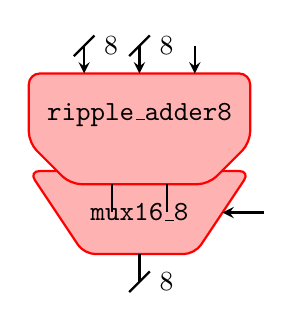
\begin{tikzpicture}[
		>=stealth,
		multiplexer/.pic={
			\coordinate (-A) at (-2em,2.5em);
			\coordinate (-B) at (2em,2.5em);
			\coordinate (-SEL) at (4.5em,0);
			\coordinate (-Q) at (0,-2.5em);
			\draw [pic actions] (-2em,-1.5em) -- (2em,-1.5em) -- (4em,1.5em) -- (-4em,1.5em) --cycle;
			\draw [->,pic actions,fill=black,draw=black] (-A) -- (-2em,1.5em);
			\draw [->,pic actions,fill=black,draw=black] (-B) -- (2em,1.5em);
			\draw [->,pic actions,fill=black,draw=black] (-SEL) -- (3em,0);
			\draw [pic actions,draw=black] (0,-1.5em) -- (-Q);
			\node [anchor=center] (-center) {\tt\tikzpictext};
	  	},
		adder/.pic={
			\coordinate (-A) at (-2em,2.5em);
			\coordinate (-B) at (0,2.5em);
			\coordinate (-Cin) at (2em,2.5em);
			\coordinate (-Cout) at (-1em,-3.5em);
			\coordinate (-S) at (1em,-3.5em);
			\draw [pic actions] (-2.5em,-2.5em) -- (2.5em,-2.5em) -- (4em,-1em) -- (4em,1.5em) -- (-4em,1.5em) -- (-4em,-1em) --cycle;
			\draw [->,pic actions,fill=black,draw=black] (-A) -- (-2em,1.5em);
			\draw [->,pic actions,fill=black,draw=black] (-B) -- (0,1.5em);
			\draw [->,pic actions,fill=black,draw=black] (-Cin) -- (2em,1.5em);
			\draw [pic actions,draw=black] (-1em,-2.5em) -- (-Cout);
			\draw [pic actions,draw=black] (1em,-2.5em) -- (-S);
			\node [anchor=center] (-center) {\tt\tikzpictext};
	  	}
	]
	\pic ["mux16\_8",thick,draw=red,fill=red!30,rounded corners] (smux) {multiplexer};

	\node [draw,strike out,thick,minimum size=0.1] (bus-S0) at (smux-A) {};
	\node [draw,strike out,thick,minimum size=0.1] (bus-S1) at (smux-B) {};
	\node [draw,strike out,thick,minimum size=0.1] (bus-S) at (smux-Q) {};
	\node [anchor=west] at (bus-S0.east) {8};
	\node [anchor=west] at (bus-S1.east) {8};
	\node [anchor=west] at (bus-S.east) {8};

	\pic ["ripple\_adder8",thick,draw=red,fill=red!30,rounded corners,above=of smux-center] (ra0) {adder};

	\node [draw,strike out,thick,minimum size=0.1] (bus-A) at (ra0-A) {};
	\node [draw,strike out,thick,minimum size=0.1] (bus-B) at (ra0-B) {};
	\node [anchor=west] at (bus-A.east) {8};
	\node [anchor=west] at (bus-B.east) {8};

	\end{tikzpicture}
	\caption{Diagram of carry ripple adder.}
\end{figure}

\begin{figure}[!h]
	\centering
	\footnotesize
	\begin{tikzpicture}
	\end{tikzpicture}
	\caption{Diagram of carry select adder.}
\end{figure}

\begin{figure}[!h]
	\centering
	\footnotesize
	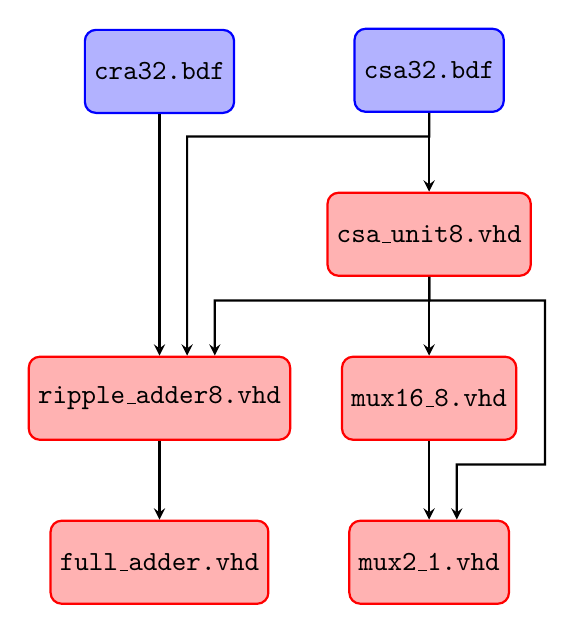
\begin{tikzpicture}[
		>=stealth,
		vhdl/.style={draw=red,fill=red!30,thick,rectangle,rounded corners,minimum size=3em},
		block/.style={draw=blue,fill=blue!30,thick,rectangle,rounded corners,minimum size=3em},
		inv/.style={draw=none,fill=none,rectangle,minimum size=3em}
	]
		\node [vhdl] (full_adder) {\texttt{full\_adder.vhd}};
		\node [vhdl,above=of full_adder] (ripple_adder8) {\texttt{ripple\_adder8.vhd}};
		\node [inv,above=of ripple_adder8] (inv) {};
		\node [block,above=of inv] (cra32) {\texttt{cra32.bdf}};

		\node [vhdl,right=of full_adder] (mux2_1) {\texttt{mux2\_1.vhd}};
		\node [vhdl,above=of mux2_1] (mux16_8) {\texttt{mux16\_8.vhd}};
		\node [vhdl,above=of mux16_8] (csa_unit8) {\texttt{csa\_unit8.vhd}};
		\node [block,above=of csa_unit8] (csa32) {\texttt{csa32.bdf}};

		\draw [->,thick] (mux16_8) -- (mux2_1);
		\draw [->,thick] (csa_unit8) -- (mux16_8);
		\draw [->,thick] (csa_unit8)
			-- ($(csa_unit8.south)!0.3!(mux16_8.north)$)
			-| ($(ripple_adder8.north) + (2em,0)$);
		\draw [->,thick] (csa_unit8)
			-- ($(csa_unit8.south)!0.3!(mux16_8.north)$)
			-| ($(mux16_8.east) + (1em,0)$)
			|- ($(mux16_8.south)!0.3!(mux2_1.north) + (1em,0)$)
			-- ($(mux2_1.north) + (1em,0)$);
		\draw [->,thick] (csa32) -- (csa_unit8);
		\draw [->,thick] (csa32)
			-- ($(csa32.south)!0.3!(csa_unit8.north)$)
			-| ($(ripple_adder8.north) + (1em,0)$);

		\draw [->,thick] (cra32) -- (ripple_adder8);
		\draw [->,thick] (ripple_adder8) -- (full_adder);
	\end{tikzpicture}
	\caption{Hierarchy of entity declarations.}
	\label{fig:hierarchy}
\end{figure}


\begin{lstlisting}[
	caption={\texttt{full\_adder\_architecture} declaration in \texttt{full\_adder.vhd}},
	label={lst:full_adder},
	language=VHDL,
	style=mystyle
]
-- architecture
ARCHITECTURE full_adder_architecture OF full_adder IS
BEGIN
	Cout <= ((A xor B) and Cin) or (A and B);
	S <= (A xor B) xor Cin;
END;
\end{lstlisting}

\begin{lstlisting}[
	caption={\texttt{mux2\_1\_architecture} declaration in \texttt{mux2\_1.vhd}},
	label={lst:mux2_1},
	language=VHDL,
	style=mystyle
]
-- architecture
ARCHITECTURE mux2_1_architecture OF mux2_1 IS
BEGIN
	Q <= (A and not SEL) or (B and SEL);
END mux2_1_architecture;
\end{lstlisting}


\begin{lstlisting}[
	caption={Snippet showing one of eight parallel \texttt{mux2\_1} components mapped in \texttt{mux16\_8.vhd} architecture declaration.},
	label={lst:mux16_8},
	language=VHDL,
	style=mystyle
]
	-- map 8 muxes with common select S
	mux0 : mux2_1 port map (A => A(0),
							B => B(0),
							SEL => SEL,
							Q => Q(0));			
\end{lstlisting}

\begin{lstlisting}[
	caption={Snippet showing one of eight chained \texttt{full\_adder} components mapped in \texttt{ripple\_adder8.vhd} architecture declaration.},
	label={lst:ripple_adder8},
	language=VHDL,
	style=mystyle
]
	SIGNAL C : std_logic_vector(6 downto 0);
BEGIN
	-- chain 8 full adders using intermediate carry signals
	fa0 : full_adder PORT MAP (	A => A(0),
								B => B(0),
								Cin => Cin,
								Cout => C(0),
								S => S(0));
\end{lstlisting}

\begin{lstlisting}[
	caption={Snippet showing how the two ripple adders were mapped to the intermediate candidate signals before being selected using multiplexors and the carry in port in \texttt{csa\_unit8.vhd} architecture declaration.},
	label={lst:csa_unit8},
	language=VHDL,
	style=mystyle
]
	-- candidates calculated by each ripple adder
	SIGNAL S0 : std_logic_vector(7 downto 0);
	SIGNAL Cout0 : std_logic;
	SIGNAL S1 : std_logic_vector(7 downto 0);
	SIGNAL Cout1 : std_logic;
BEGIN
	ra0 : ripple_adder8 PORT MAP (	A => A,
									B => B,
									Cin => '0',
									Cout => Cout0,
									S => S0);
	ra1 : ripple_adder8 PORT MAP (	A => A,
									B => B,
									Cin => '1',
									Cout => Cout1,
									S => S1);
	smux : mux16_8 PORT MAP (A => S0,
							 B => S1,
							 SEL => Cin,
							 Q => S);
	cmux : mux2_1 PORT MAP ( A => Cout0,
							 B => Cout1,
							 SEL => Cin,
							 Q => Cout);
\end{lstlisting}


\begin{figure}[!h]
	\centering
	\footnotesize
	\begin{subfigure}[b]{\textwidth}
		\makebox[\textwidth][c]{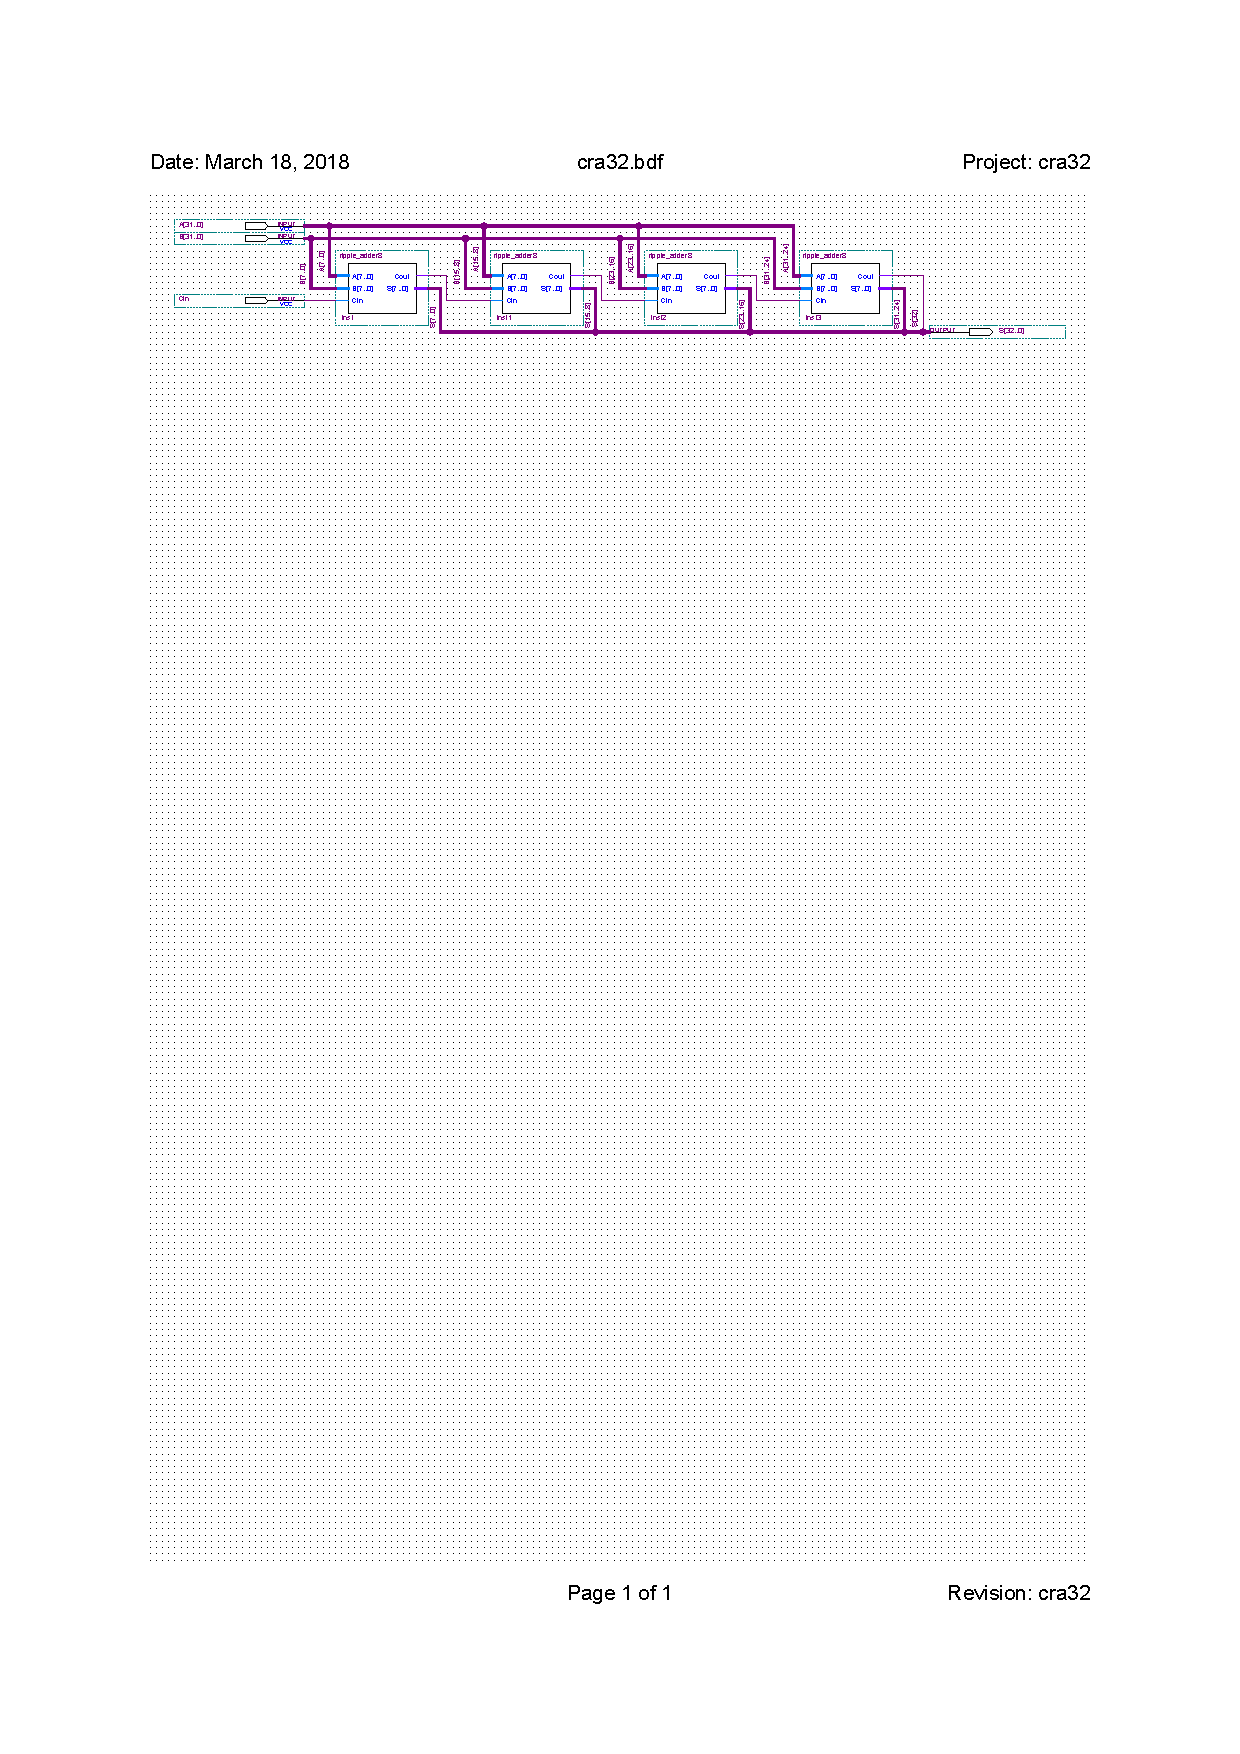
\includegraphics[width=1.3\textwidth,trim={82pt 680pt 82pt 104pt},clip]{results/cra32.pdf}}%
		\caption{\texttt{cra32.bdf}: 32-bit carry ripple adder}
		\label{fig:cra32.bdf}
	\end{subfigure}
	\begin{subfigure}[b]{\textwidth}
		\makebox[\textwidth][c]{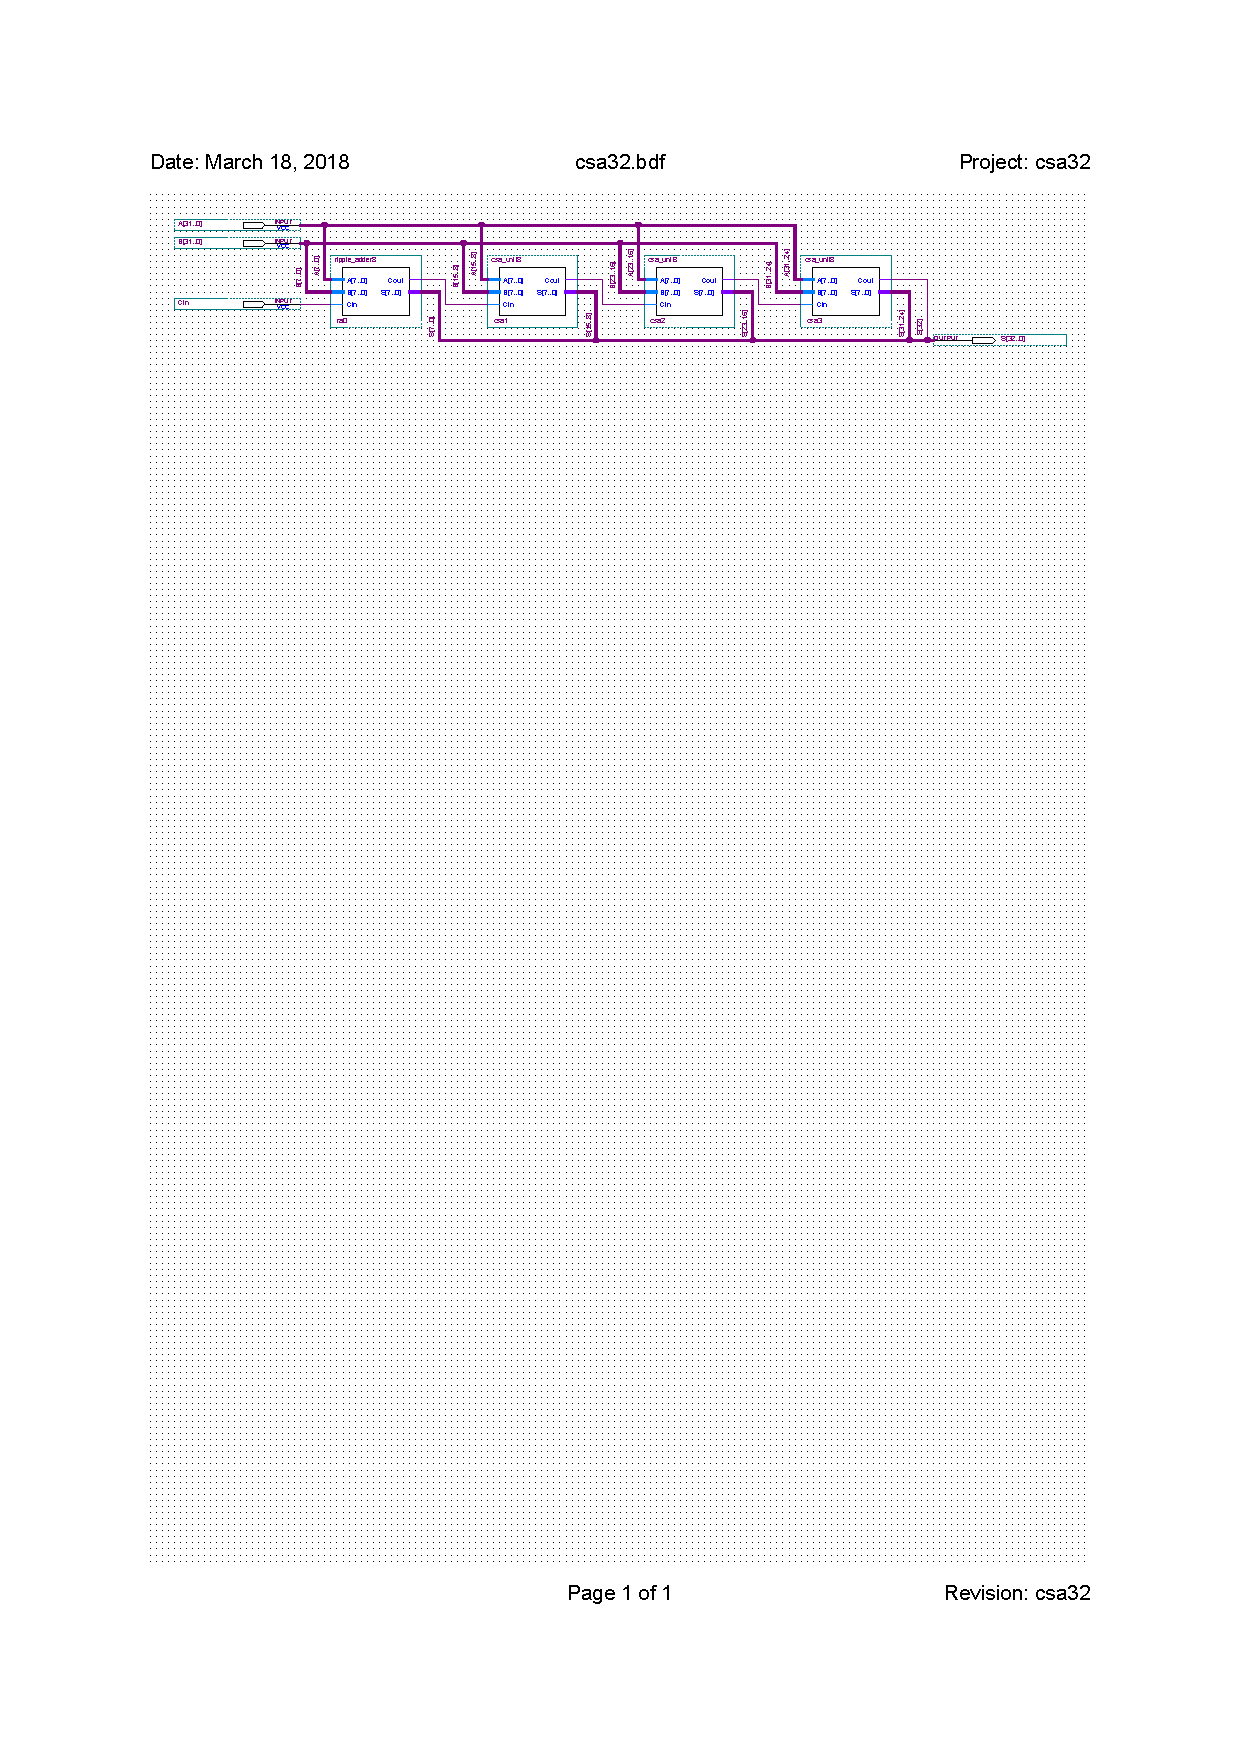
\includegraphics[width=1.3\textwidth,trim={82pt 678pt 82pt 104pt},clip]{results/csa32.pdf}}%
		\caption{\texttt{csa32.bdf}: 32-bit carry select adder, 8-bit select units}
		\label{fig:csa32.bdf}
	\end{subfigure}
	\caption{Block diagram schematics for the top-level entities of each project.}
	\label{fig:top-level}
\end{figure}

\section{Speed and Operation}

\section{FPGA Implementation}

\printbibliography

\end{document}